% (C) 2020 Diogo Rodrigues
% Licensed under Creative Commons Attribution-NonCommercial-NoDerivatives 4.0 International (CC-BY-NC-ND 4.0)

\documentclass{sope}
\usepackage[english]{babel}
% Metadata
\title{SOPE -- Exam 2014/15}
\author{Diogo Miguel Ferreira Rodrigues \\ \href{mailto:dmfrodrigues2000@gmail.com}{dmfrodrigues2000@gmail.com}}
% Document
\begin{document}

\setcounter{chapter}{14}
\exam{Exam 2014/15}
\question{Question 1}
\questionitem{Item a}
Those periods happen when a process blocks, either because it is trying to lock a resource or because it is waiting for an I/O operation to finish. The general strategy is called scheduling, and the specific technique that allows to run other processes when a process does not need the CPU is called context commuting.

\questionitem{Item b}
To resume process execution, the OS relies on the Process Control Block to retrieve all the information to restore the process exactly as it was before being paused. It requires the process ID, the process state (blocked, ready, ...), register values, priority, memory region, I/O state (open files, etc.) and other statistics like spent CPU time for other bookkeeping operations.

\questionitem{Item c}
A OS can prevent a program executing an infinite loop to indefinitely own the CPU by using a preemptive scheduling algorithm that can somehow realise it must preempt that process; for instance, the Round-Robin algorithm will periodically preempt that program to let other programs run, thus preventing other processes from starving.

\question{Question 2}
\questionitem{Item a}
To use a semaphore as if it was a mutex, one has to initialize the semaphore to 1. This is because only one lock can be made before blocking on a mutex, which means only 1 lock is initially available and a process trying to lock the mutex will have to wait for the 1 lock to be available. This is equivalent to a semaphore storing the maximum possible number of locks. As a mutex allows only 1 lock at most, the semaphore should be initialized to 1 to allow only 1 simultaneous lock to be owned by threads.

\questionitem{Item b}
A semaphore value represents the number of resources of a certain kind that can be requested (even if it is a maximum limit for the number of running threads, we can consider the \emph{number of threads that are allowed to run simultaneously} to be the resource represented by the semaphore). Thus, initializing a semaphore to a negative value means we are already saying we are using more resources than we were supposed to (as it will be necessary to signal that semaphore at least twice so a locking thread will not block; this means we are unlocking a resource we never really locked, which doesn't make sense). Given this reasonable explanation, a semaphore is probably implemented as an unsigned integer so it probably can't even have a negative value (\texttt{sem\_init} only accepts an unsigned integer actually).

\questionitem{Item c}

\textbf{c1)} This is because two operations changing an account balance at the same time is a race condition, which can lead to undefined behaviour.\\
\textbf{c2)} A careless programmer would implement a solution where a process locks the source account and then locks the destination account, then processes the transfer and the unlocks them. Imagine we want to process a transfer from A to B using process P1, and another transfer from B to A using process P2. It could happen that P1 would lock A and P2 would lock B, so P1 would block when trying to lock B and P2 would block when trying to lock A, which would cause a deadlock. 

\question{Question 3}
\questionitem{Item a}
The virtual memory seen by each process is the whole virtual memory; having $16$ pages with $\SI{1024}{\byte}$ each, the total virtual memory is $16*\SI{1024}{\byte} = \SI{16}{\mega\byte}$.

\questionitem{Item b}
Pages and frames have the same size. The physical memory has 8 frames so its total size is $8*\SI{1024}{\byte}=2^{13}\SI{}{\byte}$ so a physical address has a length of $\SI{13}{\bit}$. Virtual memory has a size of $\SI{16}{\mega\byte}=2^{14}\SI{}{\byte}$ so a virtual address has a length of $\SI{14}{\bit}$.

\questionitem{Item c}
?

\questionitem{Item d}
?

\question{Question 4}
A file is a resource for storing data in a computer storage device. A directory is a special file that allows to structure and catalogue files, by containing references to other files (directories or actual files). An i-node is the Unix struture that stores a file's metadata (permissions, owner, hard link count, etc.) and the memory blocks that are part of that file because of Unix using an indexed allocation scheme.

A file is the actual resource and the memory blocks that it is stored in, and an i-node is a struture that makes sense of a file by storing its metadata and the memory blocks it is stored in. A directory is a special file that contains a table of name/i-node pairs, where the name is what we usually call the \emph{file name} and the corresponding i-node. A directory entry referring to an i-node is called a \emph{hard link} to that file, and several directory entries (in different directories, or the same directory but with different name) can reference the same i-node.

\question{Question 5}
\questionitem{Item a}
The \emph{home} directory is the directory that contains a user's files in a multi-user operating system, and is usually of the form \texttt{/home/<user>} under Unix. The current directory is the directory the executing shell is placed at, and is usually printed in any shell prompt, usually of the form \texttt{<user>@<computer>:<path>\$} in bash under Unix. For a user there is only one home directory, while each program has its own current directory and can change it.

The user home directory can be obtained by consulting the value of the environment variable \texttt{HOME}; in the shell, using \texttt{\$HOME}, and in a C program by searching the third \texttt{main} argument or by using \texttt{getenv}.

\questionitem{Item b}

File: \texttt{exams/2015N/2015N\_05b.cpp}
\lstinputlisting[language=C,firstline=13,lastline=24,firstnumber=13]{2015N_05b.cpp}

\questionitem{Item c}
File: \texttt{exams/2015N/2015N\_05c.cpp}
\lstinputlisting[language=C,firstline=13,lastline=23,firstnumber=13]{2015N_05c.cpp}

\questionitem{Item d}
File: \texttt{exams/2015N/2015N\_05c.cpp}
\lstinputlisting[language=C,firstline=38,lastline=48,firstnumber=38]{2015N_05c.cpp}

\questionitem{Item e}
On receiving \texttt{SIGKILL}, program \texttt{list} terminates immediately and all open files are closed. Program \texttt{formatter} is not killed, because the children can continue running even after the parent is killed. \texttt{formatter} will continue reading from the pipe until it receives EOF (because the writting end has been closed when \texttt{list} was killed).

\question{Question 6}
\begin{center}
    \lstset{
        showlines=true
    }
    \begin{tabular}{c c c}
        \begin{minipage}[t]{67mm}\begin{lstlisting}[language=C]
// Use global variable
struct Data buffer[10];
        \end{lstlisting}\end{minipage} & &
        \begin{minipage}[t]{80mm}\begin{lstlisting}[language=C]
// Pass as argument
void* t1_entry(void *arg){
    struct Data *buffer =
        (struct Data*)arg;
    // ...
}
void* t2_entry(void *arg){
    struct Data *buffer =
        (struct Data*)arg;
    // ...
}
// in main
struct Data *buffer =
    calloc(10, sizeof(struct Data));
pthread_t tid1, tid2;
pthread_create(&tid1, NULL,
    t1_entry, buffer);
pthread_create(&tid2, NULL,
    t2_entry, buffer);
        \end{lstlisting}\end{minipage}
    \end{tabular}
\end{center}

\questionitem{Item b}
\begin{lstlisting}[language=C]
// Declaration, global, before the threads' functions
sem_t sem;
// Initialization, in main, before creating threads
sem_init(&sem, SEM_INI);
\end{lstlisting}

\questionitem{Item c}
The semaphore \texttt{sem} represents the number of items that have already been produced but not yet consumed. Thus, \texttt{SEM\_INI} has value 0 because initially no item has been produced.

\begin{center}
    \begin{tabular}{c c c}
        \begin{minipage}[t]{73mm}\begin{lstlisting}[language=C]
// Thread 1:
    // ...
    for(k = 0; k < 10; k++){
        fill(&buffer[k]);
        sem_post(&sem);
    }
    // ...
        \end{lstlisting}\end{minipage} & &
        \begin{minipage}[t]{73mm}\begin{lstlisting}[language=C]
// Thread 2:
    // ...
    for(k = 0; k < 10; k++){
        sem_wait(&sem);
        process(buffer[k]);
    }
    // ...
        \end{lstlisting}\end{minipage}
    \end{tabular}
\end{center}

\questionitem{Item d}
It would be possible to turn \texttt{sem} into a mutex, but it would not be very convenient because it would mean there could only be one item in the buffer that had been produced but not consumed; this could increase the program running time due to more context commutes, as it would be necessary for each item to be consumed right after it was produced. Using a semaphore, the producer can produce a bunch of items before context commute to the consumer, and the consumer could consume a bunch of items before context commute back to the producer.

\questionitem{Item e}
Having at least 2 processors, to get the minimum running time we will assume the two threads will be running each in a core at all time.

The following diagrams show what each thread is doing at each time; $f$ is the producer and $p$ is the consumer.

The producer is not limited by any synchronization mechanism, so it always takes $10t_f$.

When $t_f < t_p$, the consumer will always have something to consume because the producer can produce at a higher rate than the consumer can consume (except for the first item, for which it has to wait for $t_f$ time units), so the consumer takes $t_f + 10t_p$.

\begin{center}
    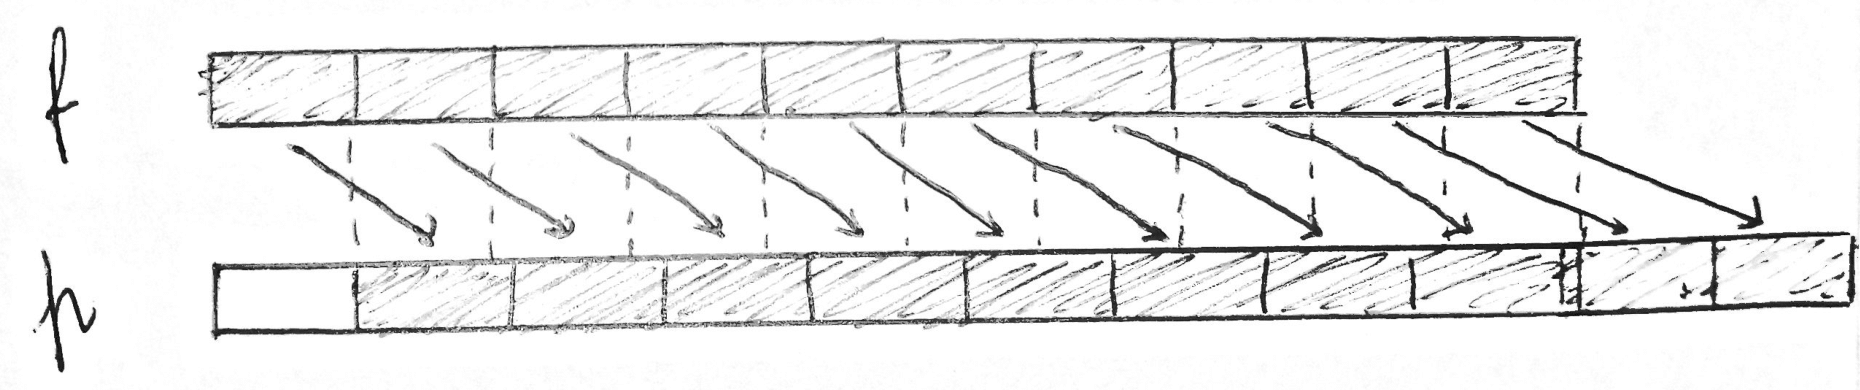
\includegraphics[scale=0.2]{2015N_06e-2}
\end{center}

When $t_f > t_p$, the consumer can consume at a higher rate than the producer can produce, so it will be blocked for $\Delta = t_f-t_p$ time units in \texttt{sem\_wait(\&sem)}; thus the consumer takes $t_f + 9(t_p+\Delta)+t_p$ (initially waits $t_f$, then consumes each of the items in $t_p$ and waits $\Delta$ for the next one, and then consumes the last one in $t_p$), which amounts to $t_f+9t_f + t_p = 10t_f + t_p$.

\begin{center}
    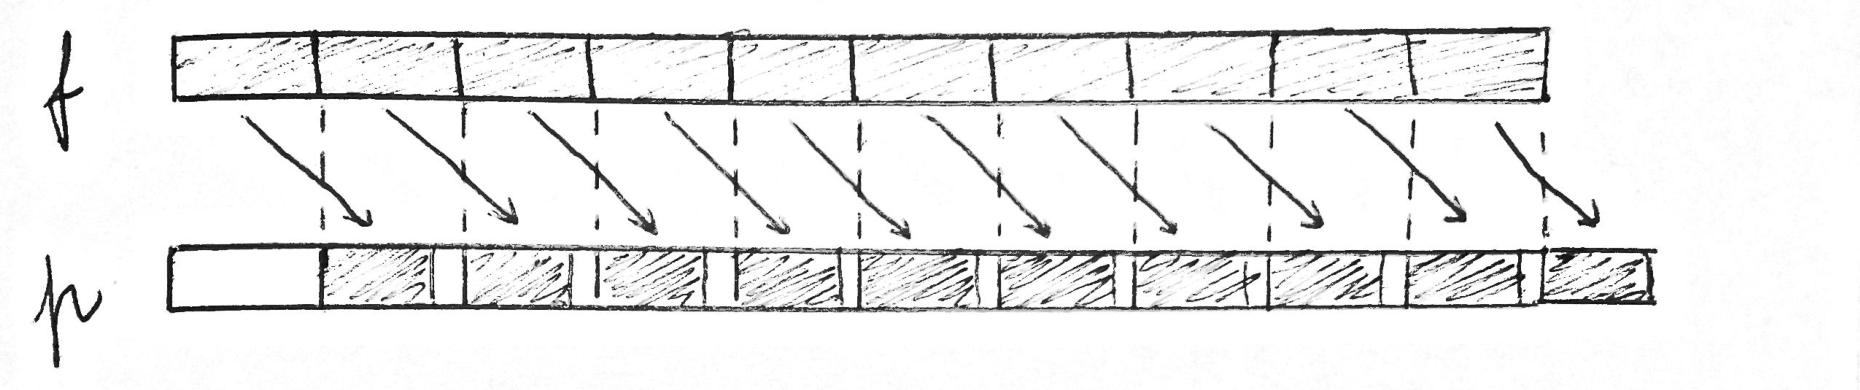
\includegraphics[scale=0.2]{2015N_06e-1}
\end{center}

\end{document}
